% CS631 Advanced Programming in the UNIX Environment
% Author: Jan Schaumann <jschauma@netmeister.org>
% $Id: slides.tex,v 1.2 2005/11/01 16:41:35 jschauma Exp $
\special{! TeXDict begin /landplus90{true}store end }

\documentclass[xga]{xdvislides}
\usepackage[landscape]{geometry}
\usepackage{graphics}
\usepackage{graphicx}
\usepackage{colordvi}

\begin{document}
\setfontphv

%%% Headers and footers
\lhead{\slidetitle}
\chead{CS631 - Advanced Programming in the UNIX Environment}
\rhead{Slide \thepage}
\lfoot{\Gray{Lecture 09: D\ae mon processes, System Logging, Shared Libraries }}
\cfoot{\relax}
\rfoot{\Gray{\today}}

\vspace*{\fill}
\begin{center}
	\Hugesize
		CS631 - Advanced Programming in the UNIX Environment\\
		-- \\
		D\ae mon processes, System Logging, Shared Libraries\\
	\hspace*{5mm}\blueline\\ [1em]
	\Normalsize
		Department of Computer Science\\
		Stevens Institute of Technology\\
		Jan Schaumann\\
		\verb+jschauma@stevens.edu+\\
		\verb+http://www.cs.stevens.edu/~jschauma/631/+
\end{center}
\vspace*{\fill}

\subsection{D\ae mon processes}
So... what's a d\ae mon process anyway?
\vfill
\hfill
\includegraphics[scale=0.5]{pics/daemon.eps} \\

\subsection{D\ae mon characteristics}
Commonly, d\ae mon processes are created to offer a specific service.
\\

D\ae mon processes usually
\begin{itemize}
	\item live for a long time
	\item are started at boot time
	\item terminate only during shutdown
	\item have no controlling terminal
\end{itemize}

\vfill
\hfill
\includegraphics[scale=0.5]{pics/daemon.eps} \\

\subsection{D\ae mon characteristics}
The previously listed characteristics have certain implications:
\\

\begin{itemize}
	\item do one thing, and one thing only
	\item no (or only limited) user-interaction possible
	\item consider current working directory
	\item how to create (debugging) output
\end{itemize}

\vfill
\hfill
\includegraphics[scale=0.5]{pics/daemon.eps} \\

\subsection{Writing a d\ae mon}
\begin{itemize}
	\item fork off the parent process
	\item change file mode mask (umask)
	\item create a unique Session ID (SID)
	\item change the current working directory to a safe place
	\item close (or redirect) standard file descriptors
	\item open any logs for writing
	\item enter actual d\ae mon code
\end{itemize}

\vfill
\hfill
\includegraphics[scale=0.5]{pics/daemon.eps} \\

\subsection{Writing a d\ae mon}
\small
\begin{verbatim}
int
daemon(int nochdir, int noclose)
{
        int fd;

        switch (fork()) {
        case -1:
                return (-1);
        case 0:
                break;
        default:
                _exit(0);
        }

        if (setsid() == -1)
                return (-1);

        if (!nochdir)
                (void)chdir("/");

        if (!noclose && (fd = open(_PATH_DEVNULL, O_RDWR, 0)) != -1) {
                (void)dup2(fd, STDIN_FILENO);
                (void)dup2(fd, STDOUT_FILENO);
                (void)dup2(fd, STDERR_FILENO);
                if (fd > STDERR_FILENO)
                        (void)close(fd);
        }
        return (0);
}
\end{verbatim}
\Normalsize

\subsection{D\ae mon conventions}
\begin{itemize}
	\item prevent against multiple instances via a {\em lockfile}
	\item allow for easy determination of PID via a {\em pidfile}
	\item configuration file convention {\tt /etc/{\em name}.conf}
	\item include a system initialization script (for {\tt /etc/rc.d/} or {\tt
		/etc/init.d/})
	\item re-read configuration file upon {\tt SIGHUP}
	\item relay information via {\em event logging}
\end{itemize}

\vfill
\hfill
\includegraphics[scale=0.5]{pics/daemon.eps} \\


\subsection{A central logging facility}

There are three ways to generate log messages:
\begin{itemize}
	\item via the kernel routine {\tt log(9)}
	\item via the userland routine {\tt syslog(3)}
	\item via UDP messages to port 514
\end{itemize}

\subsection{A central logging facility}
\begin{center}
	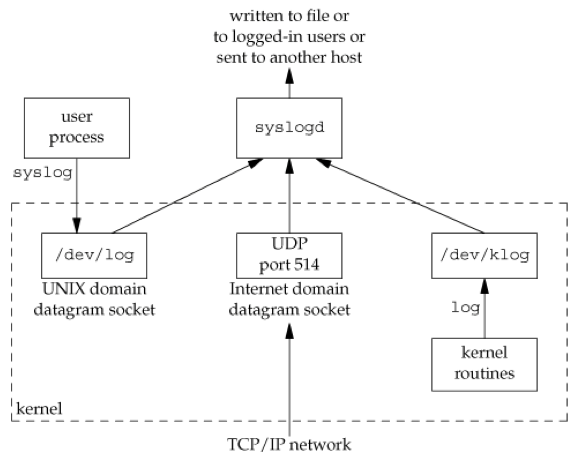
\includegraphics[scale=0.8,angle=-90]{pics/syslog.eps}
\end{center}



\subsection{\tt syslog(3)}
\small
\setlength{\unitlength}{1mm}
\begin{center}
	\begin{picture}(150,22)
		\thinlines
		\put(0,0){\framebox(130,22){}}
		\put(10,17){{\tt \#include <syslog.h>}}
		\put(10,10){{\tt void openlog(const char *{\em ident}, int {\em logopt}, int {\em facility});}}
		\put(10,5){{\tt void syslog(int {\em priority}, const char *{\em message}, ...);}}
	\end{picture}
\end{center}
\Normalsize
{\tt openlog(3)} allows us to set specific options when logging:
\begin{itemize}
	\item prepend {\em ident} to each message
	\item specify logging options ({\tt LOG\_CONS | LOG\_NDELAY | LOG\_PERRO | LOG\_PID})
	\item specify a {\em facility} (such as {\tt LOG\_DAEMON}, {\tt LOG\_MAIL} etc.)
\end{itemize}
\vspace{.5in}
{\tt syslog(3)} writes a message to the system message logger, tagged with
{\em priority}. \\
A {\em priority} is a combination of a {\em facility} (as above) and a {\em level} (such
as {\tt LOG\_DEBUG}, {\tt LOG\_WARNING} or {\tt LOG\_EMERG}).

% \subsection{Let's write a shared library, {\tt libgreet}.}
% \small
% \begin{verbatim}
% NAME
%      greet, hello, getgreeting, setgreeting — hello world library
%
% LIBRARY
%      Greetings Library (libgreet, ‐lgreet)
%
% SYNOPSIS
%      #include <greeting.h>
%
%      void greet(void);
%
%      void hello(const char * friend, const char * greeting);
%
%      char * getgreeting(void);
%
%      int setgreeting(const char * greeting);
%
% DESCRIPTION
%      The greet, family of functions allows you to easily greet your users.
%
%      The greet() function simply prints the current greeting, followed by a
%      newline character (\n) to stdout.
%
%      The hello() function prints greeting prefixed with friend, a colon (:)
%      and a space to stdout.
%
%      The getgreeting() function returns the current greeting.
%
%      The setgreeting() function sets the default greeting to use when calling
%      greet().
% \end{verbatim}
% \Normalsize
%
% \subsection{Let's write a shared library, {\tt libgreet}.}
% \begin{verbatim}
% #include <greet.h>
% #include <stdio.h>
%
% int main(void) {
%         greet();
%         if (setgreeting("Howdy!") != 0) {
%                 fprintf(stderr, "Unable to set greeting!\n");
%         }
%         greet();
%         hello("world", getgreeting());
%         return 0;
% }
% $ cc -Wall hello.c -lgreet
% $ ./a.out
% Hello!
% Howdy!
% world: Howdy!
% \end{verbatim}
% \Normalsize
%
% \subsection{Let's write a shared library, {\tt libgreet}.}
%
% \vspace{1in}
% \verb+https://www.cs.stevens.edu/~jschauma/631/f15-libgreet.html+
%
\subsection{Shared Libraries}
\begin{verbatim}
$ cat setget.c
#include <bsd/stdlib.h>
#include <stdio.h>

int
main(int argc, char **argv) {
        setprogname("setget");
        printf("My name is '%s'.\n", getprogname());
        exit(EXIT_SUCCESS);
}
$ cc -Wall setget.c
[...]
$ cc -Wall setget.c -lbsd
\end{verbatim}

\subsection{Shared Libraries}
What is a shared library, anyway?
\begin{itemize}
	\item contains a set of callable C functions (i.e., implementation
		of function prototypes defined in {\tt .h} header files)
	\item code is position-independent (i.e., code can be executed anywhere
		in memory)
	\item shared libraries can be loaded/unloaded at execution time or at will
	\item libraries may be {\em static} or {\em dynamic}
\end{itemize}

\subsection{Shared Libraries}
What is a shared library, anyway?
\begin{itemize}
	\item contains a set of callable C functions (ie, implementation
		of function prototypes defined in {\tt .h} header files)
	\item code is position-independent (ie, code can be executed anywhere
		in memory)
	\item shared libraries can be loaded/unloaded at execution time or at will
	\item libraries may be {\em static} or {\em dynamic}
\end{itemize}
\begin{verbatim}
$ man 3 fprintf
$ grep " fprintf" /usr/include/stdio.h
\end{verbatim}


\subsection{Shared Libraries}
How do shared libraries work?
\begin{itemize}
	\item contents of {\em static} libraries are pulled into the
		executable at link time
	\item contents of {\em dynamic} libraries are used to resolve
		symbols at {\bf link time}, but loaded at {\bf execution time} by the
		{\em dynamic linker}
	\item contents of {\em dynamic} libraries may be loaded at {\bf any
		time} via explicit calls to the dynamic linking loader interface
		functions
\end{itemize}

\subsection{Executable and Linkable Format}

{\bf ELF} is a file format for executables, object code, shared libraries
etc.

\begin{center}
	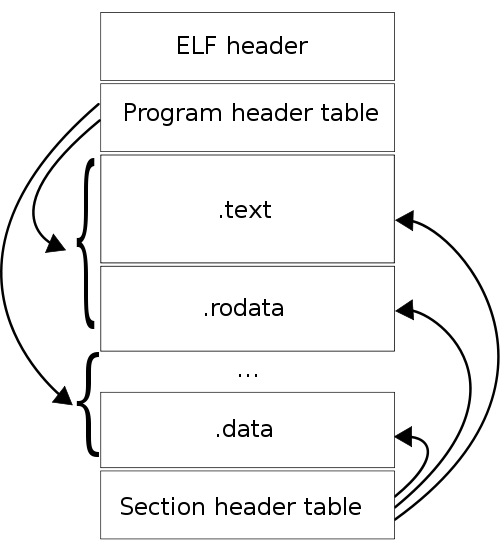
\includegraphics[scale=0.5]{pics/elf.eps}
\end{center}
More details:
\verb+http://www.cs.stevens.edu/~jschauma/631/elf.html+

\verb+http://www.thegeekstuff.com/2012/07/elf-object-file-format/+
\Normalsize


\subsection{Understanding object files}
\begin{verbatim}
$ cc -Wall -c ldtest1.c ldtest2.c main.c
$ readelf -h ldtest1.o
[...]
$ cc *.o
$ readelf -h a.out
[...]
$ ldd a.out
[...]
$ readelf -h /lib/libc.so.6
[...]
$ readelf -s a.out | more
[...]
$ objdump -d -j .text a.out | more
[...]
$ nm -D a.out | more
[...]
$
\end{verbatim}

\subsection{Statically Linked Shared Libraries}
Static libraries:
\begin{itemize}
	\item created by {\tt ar(1)}
	\item usually end in {\tt .a}
	\item contain a symbol table within the archive (see {\tt
		ranlib(1)})
\end{itemize}

\subsection{Statically Linked Shared Libraries}
\begin{verbatim}
$ cc -Wall -c ldtest1.c
$ cc -Wall -c ldtest2.c
$ cc -Wall main.c
[...]
$ cc -Wall main.c ldtest1.o ldtest2.o
$
\end{verbatim}

\subsection{Statically Linked Shared Libraries}
\begin{verbatim}
$ cc -Wall -c ldtest1.c ldtest2.c
$ ar -vq libldtest.a ldtest1.o ldtest2.o
$ ar -t libldtest.a
$ cc -Wall main.c libldtest.a

$ cc -Wall main.c -L. -lldtest -o a.out.dyn
$ cc -static main.o -L. -lldtest -o a.out.static
$ ls -l a.out.*
$ ldd a.out.*
$ nm a.out.dyn | wc -l
$ nm a.out.static | wc -l
\end{verbatim}

\subsection{Dynamically Linked Shared Libraries}
Explicit loading of shared libraries:
\begin{itemize}
	\item {\tt dlopen(3)} creates a handle for the given library
	\item {\tt dlsym(3)} returns the address of the given symbol
	\item
\end{itemize}

\begin{verbatim}
$ cc -Wall setget.c
$ cc -Wall -rdynamic dlopenex.c -ldl
$ ./a.out
\end{verbatim}

\subsection{Dynamically Linked Shared Libraries}
Dynamic libraries:
\begin{itemize}
	\item created by the compiler/linker (ie multiple steps)
	\item usually end in {\tt .so}
	\item frequently have multiple levels of symlinks providing
		backwards compatibility / ABI definitions
\end{itemize}

\subsection{Dynamically Linked Shared Libraries}
\begin{verbatim}
$ rm *.o libldtest*
$ cc -Wall -c -fPIC ldtest1.c
$ cc -Wall -c -fPIC ldtest2.c
$ mkdir lib
$ cc -shared -Wl,-soname,libldtest.so.1 -o lib/libldtest.so.1.0 ldtest1.o ldtest2.o
$ ln -s libldtest.so.1.0 lib/libldtest.so.1
$ ln -s libldtest.so.1.0 lib/libldtest.so
$ cc -static -Wall main.o -L./lib -lldtest
[...]
$ cc -Wall main.o -L./lib -lldtest
[...]
$ ./a.out
[...]
$ ldd a.out
[...]
\end{verbatim}

\subsection{Dynamically Linked Shared Libraries}
Wait, what?
\begin{verbatim}
$ export LD_LIBRARY_PATH=${LD_LIBRARY_PATH}:./lib
$ ldd a.out
[...]
$ ./a.out
[...]
$ mkdir lib2
$ cc -Wall -c -fPIC ldtest1.2.c
$ cc -shared -Wl,-soname,libldtest.so.1 -o lib2/libldtest.so.1.0 ldtest1.2.o ldtest2.o
$ ln -s libldtest.so.1.0 lib2/libldtest.so.1
$ ln -s libldtest.so.1.0 lib2/libldtest.so
$ export LD_LIBRARY_PATH=./lib2:$LD_LIBRARY_PATH
$ ldd a.out  # note: no recompiling!
[...]
$ ./a.out
[...]
\end{verbatim}

\subsection{Dynamically Linked Shared Libraries}
Avoiding {\tt LD\_LIBRARY\_PATH}:
\begin{verbatim}
$ cc -Wall main.o -L./lib -lldtest -Wl,-rpath,./lib
$ echo $LD_LIBRARY_PATH
[...]
$ ldd a.out
[...]
$ ./a.out
[...]
$ unset LD_LIBRARY_PATH
$ ldd a.out
[...]
$ ./a.out
[...]
$
\end{verbatim}

\subsection{Dynamically Linked Shared Libraries}
But:
\begin{verbatim}
$ cc -Wall -fPIC -c evil.c
$ cc -shared -Wl,-soname,libldtest.so.1 -o lib3/libldtest.so.1.0 \
        ldtest1.o ldtest2.o evil.o
$ export LD_PRELOAD=./lib3/libldtest.so.1.0
$ ldd a.out
[...]
$ ./a.out 2>/dev/null
[...]
$
\end{verbatim}

\subsection{Dynamically Linked Shared Libraries}
\begin{verbatim}
$ export LD_DEBUG=help # glibc>=2.1 only
$ ./a.out
[...]
$ LD_DEBUG=all ./a.out
[...]
\end{verbatim}

\subsection{Homework}
\verb+https://www.cs.stevens.edu/~jschauma/631/f16-libgreet.html+ \\

\begin{verbatim}
$ cat hello.c
#include <stdio.h>
#include "greet.h"

int main(void) {
        greet();
        if (setgreeting("Howdy!") != 0) {
                fprintf(stderr, "Unable to set greeting!\n");
        }
        greet();
        hello("world", getgreeting());
        return 0;
}
$ cc -Wall hello.c -I./libgreet -L./libgreet -Wl,-rpath,./libgreet -lgreet
\end{verbatim}

\end{document}
